% ----- formatovani dokumentu -----------------------------------------------
\documentclass[12pt,a4paper,titlepage,final]{report}
\usepackage[utf8]{inputenc}
\usepackage[T1, IL2]{fontenc}
\usepackage{graphicx}
\usepackage{epstopdf}
\usepackage[margin=2cm]{caption}
\usepackage[top=3cm, left=2cm, right=2cm, text={17cm, 24cm}, ignorefoot]{geometry}
\usepackage{color}
\usepackage{url}
\usepackage{setspace}
\singlespacing
\usepackage[square, numbers]{natbib} 
\pagestyle{plain}
\pagenumbering{arabic}
\setcounter{page}{1}
\setcounter{secnumdepth}{-1}
\setlength{\parindent}{1cm}	
\usepackage{natbib}


% ----- vyberte jazyk -------------------------------------------------------
\usepackage[english,czech]{babel}
%\usepackage[english]{babel}

% ----- dopiste titulky -----------------------------------------------------
\newcommand\Course{Počítačová grafika}
\newcommand\WorkTitle{Téma semestrální práce}
\newcommand\AuthorA{Zdeněk Biberle}
\newcommand\AuthorAEmail{xbiber00@stud.fit.vutbr.cz}
\newcommand\AuthorB{Tomáš Šujan}
\newcommand\AuthorBEmail{xsujan02@stud.fit.vutbr.cz}
\newcommand\AuthorC{Zdeněk Tretter}
\newcommand\AuthorCEmail{xtrett00@stud.fit.vutbr.cz}
\newcommand\Faculty{Fakulta Informačních Technologií}
\newcommand\School{Vysoké Učení Technické v Brně}

\usepackage[
pdftitle={\WorkTitle},
pdfauthor={\AuthorA, \AuthorB, \AuthorC},
bookmarks=true,
colorlinks=true,
breaklinks=true,
urlcolor=blue,
citecolor=blue,
linkcolor=blue,
unicode=true,
]
{hyperref}


% ----- titulni strana ------------------------------------------------------

\begin{document}
	\begin{titlepage}
	\begin{center}
		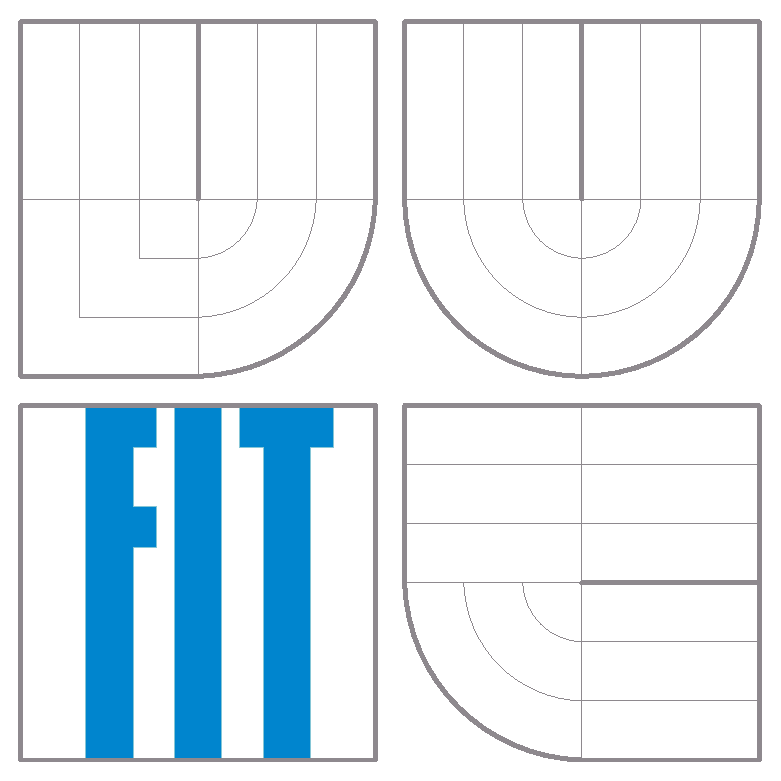
\includegraphics[height=5cm]{images/logo.eps}
	\end{center}
	\vfill
	\begin{center}
		\begin{Large}
			\Course\\
		\end{Large}
		\bigskip
		\begin{Huge}
			\WorkTitle\\
		\end{Huge}
	\end{center}
	\vfill
	\begin{center}
		\begin{large}
			\today
		\end{large}
	\end{center}
	\vfill
	\begin{flushleft}
		\begin{large}
			\begin{tabular}{lll}
				Autoři: & \AuthorA, & \url{\AuthorAEmail} \\
				        & \AuthorB, & \url{\AuthorBEmail} \\
				        & \AuthorC, & \url{\AuthorCEmail} \\
				& & \\
				& \Faculty \\
				& \School \\
			\end{tabular}
		\end{large}
	\end{flushleft}
\end{titlepage}		
	
% ----- obsah --------------------------------------------------------------
	
\tableofcontents

% ----- zadani -------------------------------------------------------------
\newpage
\chapter{Zadání}

Zde napište informace k zadání (nejde jen o přepis toho, co je na webu;
komentujte vaše vlastní zpřesnění zadání, zaměření, důrazy, pojetí atd.). Text
strukturujte, použijte odrážky, číslování$\ldots$

\paragraph{Rozsah:} cca 10 odrážek

\begin{itemize}
	\item Položka 1
	\begin{itemize}
		\item Podpoložka 1.1
		\item Podpoložka 1.2
		\item $\ldots$
	\end{itemize}
	\item Položka 2
	\begin{itemize}
		\item Podpoložka 2.1
		\item Podpoložka 2.2
		\item $\ldots$
	\end{itemize}
	\item $\ldots$
\end{itemize}

%---------------------------------------------------------------------------
\chapter{Nejdůležitější dosažené výsledky}

Popište 3 věci, které jsou na vašem projektu nejlepší. Nejlépe ukažte a
komentujte obrázky, v nejhorším případě vypište textově.

\section{První věc}

Lorem ipsum dolor sit amet, consectetur adipiscing elit. In non condimentum augue, quis accumsan tellus. Sed sagittis mauris tortor, a varius ipsum feugiat sed. Morbi dapibus neque purus, id condimentum sem tincidunt quis. Sed lacinia a justo in rutrum. Nam a enim id urna cursus consectetur non a mi. Fusce vitae augue urna. Nunc nec malesuada enim, vitae blandit leo. Vestibulum et orci nibh. Phasellus in nisi rutrum, mattis metus vehicula, tempus neque.

\begin{itemize}
	\item Položka 1
	\begin{itemize}
		\item Podpoložka 1.1
		\item Podpoložka 1.2
		\item $\ldots$
	\end{itemize}
	\item Položka 2
	\item $\ldots$
\end{itemize}

%\begin{center}
%	\captionsetup{type=figure}
%		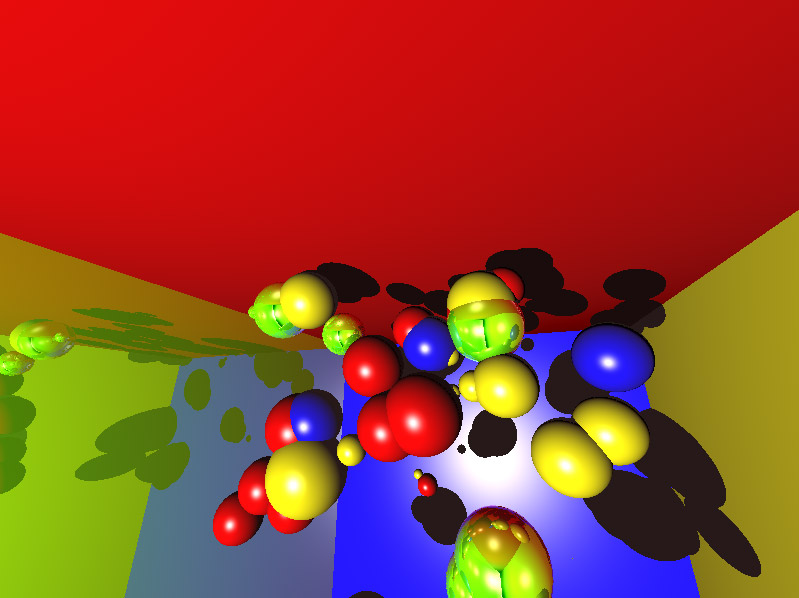
\includegraphics[width=10cm]{images/sample.jpg}
%	\captionof{figure}{Popisek vzorového obrázek}
%\end{center}

\section{Druhá věc}

Etiam a laoreet dolor, vel blandit ipsum. Pellentesque habitant morbi tristique senectus et netus et malesuada fames ac turpis egestas. Nam aliquet ipsum eget semper pretium. Maecenas mauris tortor, pretium sit amet convallis et, iaculis vel tortor. Donec ultrices magna et commodo tempus. Etiam sagittis lectus vitae lectus ultricies tincidunt. Nam aliquam non magna eget pellentesque. 

\begin{table}[h!]
	\begin{center}
    \begin{tabular}{ | p{3.5cm} | p{3.5cm} | p{3.5cm} | p{3.5cm} |}
    \hline
    Sloupec A & Sloupec B & Sloupec C & Sloupec D
    \\ \hline
    
	A1 & B1 & C1 & D1
	\\ \hline
	
	A2 & B2 & C2 & D2
	\\ \hline
	
    \end{tabular}
	\end{center}	
	\caption{Vzorová tabulka}  
\end{table}

\section{Třetí věc}
  	Jednoduchá a přesto slušně uvěřitelná textura mraků, které se navíc pohybují a mění.
    TODO obrázek
    
  


%---------------------------------------------------------------------------
\chapter{Zvláštní použité znalosti}

Uveďte informace, které byly potřeba nad rámec výuky probírané na FIT.
Vysvětlete je pomocí obrázků, schémat, vzorců apod. 

\paragraph{Rozsah:} podle potřeby a vlastního uvážení


%---------------------------------------------------------------------------
\chapter{Práce na projektu}

\begin{itemize}
\item \textbf{\AuthorA}: Aplikace, zpracování a UV mapování modelů, obecné shadery, textury drevo.glsl, kamuflaz.glsl a digitalnikamuflaz.glsl
\item \textbf{\AuthorB}: Textura dlazba.glsl
\item \textbf{\AuthorC}: Textury kachlicky.glsl, jeansy.glsl, mraky.glsl a mrakyNaHladine.glsl
\end{itemize}

%---------------------------------------------------------------------------
\section{Co bylo nejpracnější}

\begin{itemize}
\item \textbf{\AuthorA}: Jelikož doplnění textur o normálové mapy byl původně můj nápad, tak také bylo na mě, abych tuto techniku implementoval. Až později jsem ovšem zjistil, že pro mapování normál nestačí znát pouze normálové vektory jednotlivých vrcholů modelu, ale je nutné mít k dispozici celý tangentní prostor. Poté jsem začal experimentovat s výpočtem tangentního prostoru pomocí knihovny Open Asset Import Library i mého vlastního řešení. Nakonec kombinací obou metod dorazil k řešení, které stále není ideální, ale obecně funguje poměrně obstojně.
\item \textbf{\AuthorB}: Najpracnejšou časťou projektu bola z môjho pohľadu konsolidácia návrhu textúry do samotného fragment shaderu. Svoje teoretické nápady na procedurálnu generáciu textúr som musel niekoľkokrát pozmeniť. Výsledkom môjho prvotného návrhu bola nekvalitná textúra.  Algoritmus výpočtu šumu som pozmenil a vytvoril som novú textúru znázorňujúcu bunkovú štruktúru, no oba výsledky boli tentoraz fádne a jednoliate. Nakoniec som tieto dva návrhy zlúčil do jedného. Výsledná textúra má relatívne komplexný vzhľad aj za použitia normál, ktorý by dve textúry samy o sebe určite nedosiahli. Jednu dobu sa na kockách objavovali grafické artefakty, ktoré boli spôsobené nekorektným otočením normálovéhu uhlu - na nesprávnu stranu. Pracné bolo teda vymyslieť také riešenie, aby moja dovtedajšia práca nebola stratená, ale zároveň, aby výsledkom bola relatívne kvalitná textúra, ktorá bude mať aj určitú priestorovú komplexnosť.
\item \textbf{\AuthorC}: Největším problémem u mě bylo projekt přeložit, abych mohl začít pracovat. Na windows se mi nedařilo správně nainstalovat všechny potřebné knihovny a vše správně nastavit. Linux zase nechtěl spolupracovat s mojí AMD grafikou. A integrovaná grafika nepodporovala vyšší verze OpenGL. Nakonec jsem programoval přes VNC u Zdeňka Biberleho. 

Co se týče samotného programování, tak nebylo jednoduché odhadnout, jak se jednotlivé OpenGL funkce zachovají na různé vstupy. O to složitější to bylo při jejich kombinaci, proto jsem měl vždy na začátku jen základní představu, jak by měla výsledná textura vypadat. Postupně jsem pak vymýšlel detaily, jejichž implementace si ale mnohdy vyžádala i značné změny již napsaného kódu, což bylo časově náročné. 

\end{itemize}


%---------------------------------------------------------------------------
\section{Zkušenosti získané řešením projektu}

\begin{itemize}
	\item 
\end{itemize}

Popište, co jste se řešením projektu naučili. Zahrňte dovednosti obecně
programátorské, věci z oblasti počítačové grafiky, ale i spolupráci v týmu,
hospodaření s časem, atd.

\paragraph{Rozsah:} formulujte stručně, uchopte cca 3-5 věcí

\begin{itemize}
\item \textbf{\AuthorA}:
\item \textbf{\AuthorB}:
\item \textbf{\AuthorC}: Seznámení s jazykem GLSL, programování v něm, poznání čeho je schopen a práce přes VNC.
\end{itemize}

%---------------------------------------------------------------------------
\chapter{Autoevaluace}

\paragraph{Technický návrh (80\%):} Celý projekt je poměrně vhodně rozdělen na jednoduché podproblémy a zpravidla se jedná o platformu vhodnou pro experimentování s generováním různě složitých procedurálních textur.

\paragraph{Programování (80\%):} Z tohoto pohledu je aplikace kvalitně zpracovaná, ovšem místy je slabě komentovaná. To je zjevné primárně u zdrojových kódů samotných textur, které jsou plné zdánlivě náhodně použitých funkcí a magických konstant.

\paragraph{Vzhled vytvořeného řešení (75\%):} Estetická kvalita je přijatelná, ale rozhodně ne dokonalá. Bylo by možné ji vylepšit například lepším mapováním textur na zvolené modely.

\paragraph{Využití zdrojů (60\%):} Bylo využito několik zdrojů týkajících se primárně generování šumu, a to jak kód, tak i teoretické základy. Obecně mohlo být zdrojů použito více.

\paragraph{Hospodaření s časem (50-90\%):} Práce na projektu začala dokonce i dříve, než byl projekt oficiálně zaregistrován. I přesto byly činnosti přiřazené některým členům týmu dokončeny později, než bylo očekáváno. Ale i přesto je projekt dokončen a nemá žádné výrazné nedostatky.

\paragraph{Spolupráce v týmu (50\%):} Zdena a Tomáš se mohli míň flákat a aspoň si to rozjet :P. TODO DOPLNIT

\paragraph{Celkový dojem (50\%):} Práce na tomto projektu byla příjemnou zkušeností, a to primárně z toho důvodu, že se jednalo hlavně o artistickou činnost, u které je člověk omezen jenom svou představivostí. BLAH BLAH BLAH TODO.

%---------------------------------------------------------------------------
\chapter{Ovládání vytvořeného programu}

\section{Technologie potřebné pro spuštění programu}
\paragraph{Softwarové púožadavky}
\begin{itemize}
	\item Knihovna SDL2 - Vytvoření a ovládání okna aplikace a OpenGL kontextu.
	\item Knihovna GLEW - Nahrávání OpenGL funkcí
	\item Knihovna Open Asset Import Library - Nahrávání modelů.
\end{itemize}

\paragraph{Hardwarové požadavky}
\begin{itemize}
	\item Grafická karta s podporou alespoň OpenGL 3.3
\end{itemize}

\section{Programy a služby použité při tvorbě}
\begin{itemize}
	\item Blender - Úprava a tvorba modelů a mapování textur.
\end{itemize}

\section{Obsluha programu}
\begin{itemize}
	\item Držení levého tlačítka myši - Společně s pohybem myši umožňuje rotaci modelu.
	\item Kolečko myši - Přiblížení a oddálení modelu.
	\item Klávesa F5 - Opětovné nahrání a zkompilování shaderů.
	\item Klávesa R - Zapíná a vypíná autonomní rotaci modelu.
	\item Klávesa T - Zapíná a vypíná zobrazení tangentního prostoru modelu.
	\item Šipka doleva a doprava - Přepíná mezi texturovacími shadery.
	
	
\end{itemize}

%---------------------------------------------------------------------------
\chapter{Doporučení pro budoucí zadávání projektů}

Co vám vyhovovalo a co nevyhovovalo na organizaci projektů? Které prvky by měly být zachovány, zesíleny, potlačeny, eliminovány?

%---------------------------------------------------------------------------

\chapter{Různé}

Ještě něco by v dokumentaci mělo být? Napište to sem! Podle potřeby i založte
novou kapitolu.

%---------------------------------------------------------------------------

\bibliographystyle{plain}

\nocite{cite1}
\nocite{cite2}
\nocite{cite3}
            
\bibliography{reference}
\addcontentsline{toc}{chapter}{Literatura}

\end{document}

